Históricamente, la seguridad constituyó una de las principales debilidades del protocolo SNMP. Las primeras versiones fueron diseñadas con un fuerte énfasis en la simplicidad y la interoperabilidad, relegando aspectos relacionados con la autenticación, la confidencialidad y el control de acceso. Como consecuencia, durante muchos años SNMP fue utilizado principalmente para tareas de monitorización, mientras que las funciones de configuración remota eran empleadas con mayor cautela.

\subsection{Debilidades de Seguridad en SNMPv1 y SNMPv2c}

Las versiones SNMPv1 y SNMPv2c carecen de mecanismos de seguridad robustos. La autenticación se basa en el uso de \textit{community strings}, que funcionan como contraseñas compartidas entre el \textit{Manager} y el \textit{Agent}.

El principal problema de este enfoque es que dichas credenciales son transmitidas en texto plano dentro de los mensajes SNMP. En consecuencia, un atacante con acceso al tráfico de red puede capturar fácilmente las \textit{community strings} mediante herramientas de análisis de paquetes y utilizarlas para acceder al dispositivo gestionado.

Esta limitación redujo considerablemente la confianza en las operaciones de modificación remota. En muchos entornos productivos, las operaciones \textit{SetRequest} fueron deshabilitadas o restringidas para evitar cambios no autorizados en la configuración de los equipos.

\subsection{User-Based Security Model (USM)}

Con la aparición de SNMPv3 se introdujo una arquitectura de seguridad diseñada para resolver las limitaciones de las versiones anteriores. El componente central de esta arquitectura es el \textit{User-Based Security Model} (USM).

A diferencia del modelo basado en comunidades, USM utiliza identidades de usuario para determinar los permisos y servicios de seguridad aplicables a cada operación. De esta forma, las solicitudes son asociadas a usuarios específicos en lugar de depender de una única credencial compartida.

USM proporciona mecanismos de autenticación, integridad y confidencialidad para los mensajes intercambiados entre gestores y agentes, permitiendo verificar el origen de las comunicaciones y proteger la información transmitida frente a accesos no autorizados.

\subsection{Autenticación y Cifrado en SNMPv3}

La seguridad de SNMPv3 se apoya en mecanismos criptográficos destinados a garantizar tanto la autenticidad de los mensajes como la privacidad de la información intercambiada.

\subsubsection{Autenticación}

La autenticación se implementa mediante algoritmos basados en HMAC (\textit{Hash-Based Message Authentication Code}), los cuales permiten verificar que un mensaje proviene de una fuente legítima y que no ha sido modificado durante la transmisión.

Entre los algoritmos más utilizados se encuentran MD5 y SHA, siendo este último el preferido en implementaciones modernas debido a sus mayores garantías de seguridad.

Además de verificar la integridad de los datos, estos mecanismos ayudan a prevenir ataques de repetición y otras formas de manipulación de mensajes.

\subsubsection{Cifrado y Privacidad}

SNMPv3 también incorpora servicios de privacidad mediante el cifrado de los mensajes intercambiados entre gestores y agentes.

El cifrado impide que terceros puedan interpretar el contenido de las comunicaciones incluso cuando logren capturar los paquetes transmitidos por la red.

Históricamente, el algoritmo más utilizado fue DES (\textit{Data Encryption Standard}). Sin embargo, las implementaciones actuales suelen emplear AES (\textit{Advanced Encryption Standard}), que proporciona un nivel de seguridad significativamente superior.

\begin{figure}[H]
\centering
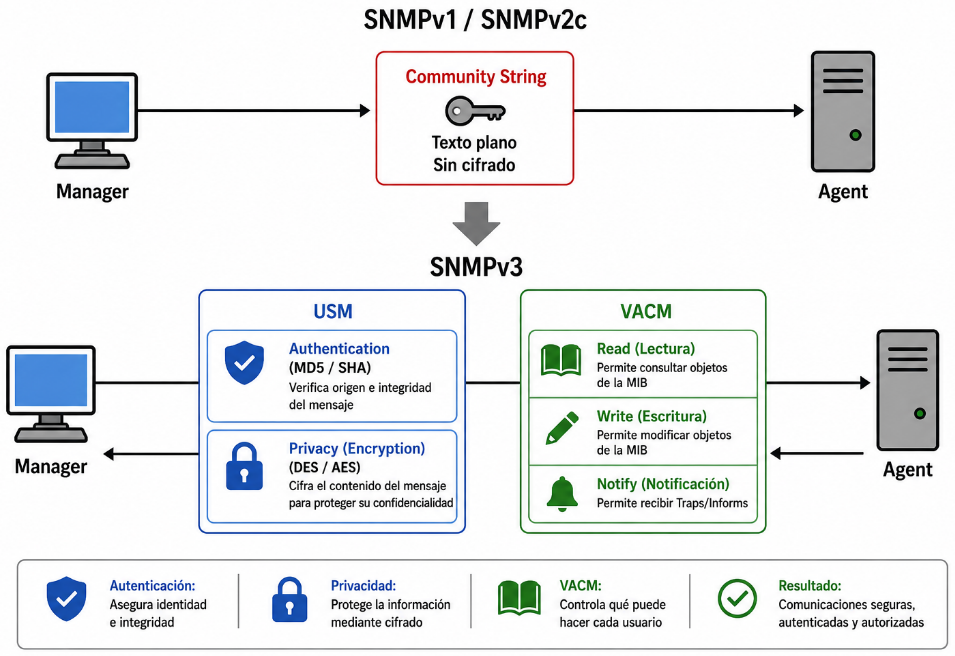
\includegraphics[width=0.8\textwidth]{img/snmp3.png}
\caption{Mecanismos de autenticación y cifrado incorporados en SNMPv3 para proteger las comunicaciones entre gestores y agentes.}
\label{fig:snmpv3_seguridad}
\end{figure}

\subsection{Control de Acceso y Buenas Prácticas}

La protección de una infraestructura SNMP no depende únicamente de la autenticación y el cifrado. También es necesario controlar qué recursos puede consultar o modificar cada usuario.

\subsubsection{View-Based Access Control Model (VACM)}

El \textit{View-Based Access Control Model} (VACM) complementa a USM proporcionando mecanismos de autorización granular sobre los objetos de la MIB.

Mediante VACM es posible definir vistas específicas de la información disponible y asociarlas a distintos usuarios o grupos. De esta manera, ciertos gestores pueden tener acceso únicamente de lectura, mientras que otros pueden disponer de permisos adicionales para realizar modificaciones sobre determinados objetos.

Este modelo permite aplicar el principio de mínimo privilegio, reduciendo la superficie de exposición ante errores operativos o accesos indebidos.

\subsubsection{Buenas Prácticas de Implementación}

Además de las capacidades de seguridad incorporadas por SNMPv3, se recomienda adoptar medidas complementarias a nivel de infraestructura para reducir riesgos operativos.

Una práctica habitual consiste en aislar el tráfico de administración dentro de VLANs de gestión dedicadas, separándolo del tráfico de usuarios y aplicaciones.

Asimismo, resulta recomendable implementar listas de control de acceso (ACLs) que limiten la comunicación SNMP exclusivamente a las estaciones de gestión autorizadas. Estas restricciones permiten reducir significativamente la exposición de los puertos UDP 161 y UDP 162 frente a intentos de acceso no autorizados.

La combinación de SNMPv3, mecanismos de control de acceso y una adecuada segmentación de red constituye actualmente la estrategia más utilizada para proteger entornos de monitorización y administración de infraestructura.
